% =====================================================================
% MIBEL Congestion Monitor v3 — Working paper (English edition)
% Author: Carlo Vilches
% Compile: pdflatex Memoria_MIBEL_v2.tex
%          bibtex   Memoria_MIBEL_v2
%          pdflatex Memoria_MIBEL_v2.tex
%          pdflatex Memoria_MIBEL_v2.tex
% =====================================================================

\documentclass[11pt,a4paper]{article}

\usepackage[utf8]{inputenc}
\usepackage[T1]{fontenc}
\usepackage[english]{babel}
\usepackage{lmodern}
\usepackage[a4paper, margin=2.5cm]{geometry}
\usepackage{booktabs}
\usepackage{array}
\usepackage{multirow}
\usepackage{tabularx}
\usepackage{caption}
\usepackage{subcaption}
\usepackage{graphicx}
\usepackage{float}
\usepackage{amsmath, amssymb}
\usepackage{siunitx}
\usepackage{xcolor}
\usepackage[colorlinks=true, linkcolor=blue, citecolor=blue, urlcolor=blue]{hyperref}
\usepackage[round, authoryear]{natbib}
\usepackage{enumitem}
\usepackage{microtype}

\setlist{nosep}
\sisetup{detect-weight=true, group-separator={\,}}
\graphicspath{{../plots/}}

\title{\textbf{Anomaly detection in the Spain--France Day-Ahead spread
of the Iberian Electricity Market:\\
a residual-based surveillance system with honest evaluation
on open data (2019--2024)}}
\author{Carlo Vilches\thanks{Working paper, version \texttt{v3.2}, 2026-05.
The Spanish predecessor (\texttt{v1}, 2025) is preserved in
\texttt{docs/Memoria\_MIBEL\_CarloVilches.pdf}; the present version
incorporates a systematic post-hoc audit that corrected leakage in
rolling features and in the régime-specific pooled comparison,
together with the alignment of regulatory dates to the entry into force
of Royal Decree-law 10/2022 (15 June 2022).}}
\date{\today}

\begin{document}

\maketitle

\begin{abstract}
\noindent
We construct a residual-based surveillance system for the Day-Ahead
electricity spread between Spain and France in the Iberian Electricity
Market (MIBEL), over 2019--2024 ($n = 52\,530$ hourly observations),
using exclusively open data. The architecture separates the
\emph{fundamentals} model from the \emph{detection} module: an XGBoost
\emph{ex ante} predictor estimates the expected spread, and the
residuals feed a Verde/Ámbar/Naranja/Roja (Green/Amber/Orange/Red)
cascade based on a 168-hour rolling \emph{z-score} with mandatory
\texttt{shift(1)}. On the 2024 test set (out-of-sample, post-Iberian-
Exception) the model achieves $R^2 = 0{,}539$ and
$\mathrm{RMSE} = 3{,}22$~€/MWh. The XGBoost achieves lower RMSE than
the competitive econometric benchmarks AR(1), AR(24) and LASSO with
cross-validation, but with $n = 8\,783$ the Diebold--Mariano test does
not reach 5\% significance against these competitors
($p \in [0{,}06;\,0{,}12]$). Statistical significance is maintained
against the naive benchmarks (persistence and zero level,
$p < 10^{-3}$). The system is validated systematically against a
pre-specified panel of 40 documented events: 83\% of the 24 in-window
events (2022--2024) are detected, against 75\% from a naive
$|\text{spread}| > p_{99}$ régime-specific benchmark; the McNemar test
on paired discordant cells does not reach 5\% significance with
$n = 24$ ($p = 0{,}50$). Régime-specific models outperform the unified
pooled specification by an ample margin in the Crisis-and-Iberian-
Exception regime ($-18{,}1\%$ RMSE) and produce a tie ($< 2\%$ RMSE) in
the pre-crisis and post-exception regimes; the hypothesis of dominant
transfer learning across regimes is therefore rejected. We further
report an operational calibration analysis (Pareto frontier across 100
threshold combinations) showing that the default cascade lies above
the elbow of the precision-coverage trade-off and admits a five-fold
reduction in alert volume while preserving recall and improving
precision@72h from 0.148 to 0.212. The system positions itself as a
quantitative screening layer for REMIT~II-grade surveillance; as a
stand-alone tool it does not satisfy ACER's transaction-reporting
requirements.
\end{abstract}

% =====================================================================
\section{Introduction and objectives}
% =====================================================================

The Iberian Electricity Market (MIBEL) operates under a market-coupling
mechanism with the rest of Europe through the Spain--France
interconnection. When commercial Available Transfer Capacity (ATC) is
sufficient, prices on both sides of the border converge; when the
interconnection saturates, the markets decouple and a price differential
or \emph{spread} emerges, reflecting the physical congestion of the
grid. The European electricity-integration literature \citep{Newbery2016}
documents the welfare gains from such convergence and the costs
associated with its loss during congestion episodes.

The objective of this work is to construct a \textbf{residual-based
surveillance system} for the Day-Ahead (DA) Spain--France spread. The
architecture separates the \emph{estimation} of the expected market
behaviour from the \emph{detection} of anomalies. An economic
fundamentals model (XGBoost, \emph{ex ante}) predicts the expected
spread given the state of the system; the residual between the
observed and predicted spread is used as an operational signal.
Episodes with residuals that are persistently large in magnitude
\emph{relative} to the recent volatility of the same regime signal
deviations that cannot be explained by the observed fundamentals.
Parametric modelling of spread risk has precedents in \citet{Bunn2016}.

The system positions itself as a complementary indicator that could
be integrated into surveillance pipelines under REMIT~II. As a
stand-alone tool it \textbf{does not} satisfy ACER's transaction-
reporting requirements \citep{ACER2024}, which demand granular
bid-ask data, order-book information and REMIT transaction reports
not consumed by this model. The connection with regulation is
therefore operational and limited, not exhaustive.

This version refines two aspects of the initial release: the dating
of the regulatory regimes (following the actual entry into force of
Royal Decree-Law~10/2022, 15 June 2022) and the alignment between
the methodology described and the code implementation, including the
correction of three leakage and calibration issues uncovered by a
systematic post-hoc audit (see Note on revised metrics at the
beginning of Section~\ref{sec:results}).

% =====================================================================
\section{Data and methodology}
% =====================================================================

\subsection{Data sources and licensing}

The project uses exclusively open data sources. The final dataset
covers 2019-01-01 to 2024-12-31, $n = 52\,530$ hourly observations
after dropping rows with null target or key lag.

\begin{table}[H]
\centering
\small
\caption{Data sources.}
\label{tab:fuentes}
\begin{tabularx}{\linewidth}{lXll}
\toprule
\textbf{Variable} & \textbf{Source} & \textbf{Resolution} & \textbf{Access} \\
\midrule
DA prices ES/FR        & OMIE                & Hourly  & Public (direct download) \\
Intraday prices        & OMIE                & Hourly  & Public (direct download) \\
NTC ES$\leftrightarrow$FR & JAO SWE CCR      & Hourly  & Public (REST API, no token) \\
TTF gas price          & Yahoo Finance       & Daily   & Public (\texttt{yfinance}) \\
CO$_2$ EUA allowances  & Yahoo Finance       & Daily   & Public (\texttt{yfinance}) \\
\bottomrule
\end{tabularx}
\end{table}

\paragraph{Caveat on yfinance.} The use of \texttt{yfinance} for TTF
and EUA series is convenient for reproducibility but is \emph{not} a
primary regulatory source: Yahoo Finance is an aggregator and its
terms of service limit systematic scraping. The official TTF series
are hosted at Euronext/EEX and the EUA series at ICE Endex; a
serious operational deployment would require a subscription to one
of those sources. The pipeline raises an explicit error if the
downloader returns empty data; silent fallbacks to synthetic series
are disabled.

\subsection{Regulatory regimes}

A relevant methodological contribution is the correct dating of the
regulatory regimes. Version \texttt{v1} used a calendar cut-off
(1 January 2022) that mixes the pre-gas-cap crisis (Russian invasion
of Ukraine, 24 February 2022) with the Iberian Exception (which
entered into force on 15 June 2022 via Royal Decree-Law~10/2022 and
ended on 31 December 2023). For sample-size reasons (the
``crisis-without-cap'' sub-regime would have $\approx 3\,960$ hours
only) we consolidate both sub-periods into a single
\texttt{crisis\_y\_excepcion} regime, but we explicitly declare the
regulatory change date and discuss its implications \citep{Fabra2023}.
The three final regimes are:

\begin{itemize}
\item \texttt{pre\_crisis}: 2019-01-01 to 2021-12-31
   ($n = 26\,253$).
\item \texttt{crisis\_y\_excepcion}: 2022-01-01 to 2023-12-31
   ($n = 17\,494$). Includes the pre-cap crisis (January--14 June 2022)
   and the Iberian Exception (15 June 2022 to 31 December 2023).
\item \texttt{post\_excepcion}: 2024-01-01 to 2024-12-31
   ($n = 8\,783$).
\end{itemize}

\subsection{System architecture and feature engineering}\label{sec:arch}

The system is organised in three sequential phases:

\begin{enumerate}
\item \textbf{Fundamentals modelling (XGBoost)} with the
``A clean'' feature set: lags of the DA spread, rolling means and
rolling volatility, energy fundamentals (TTF, CO$_2$, spark spread,
clean spark spread), NTC ES$\leftrightarrow$FR with an observability
indicator, and calendar variables. The choice of XGBoost over
classical econometric alternatives (LASSO, AR) is justified
empirically in Section~\ref{sec:bench-dm}; deep neural networks are
not explored because of their interpretability cost relative to the
expected gain at this hourly horizon \citep{Lago2018, Lago2021}.

\item \textbf{Residuals computation}:
\[
r_t = \mathrm{spread}_\text{DA}^\text{obs}(t) - \widehat{\mathrm{spread}}_\text{DA}(t).
\]

\item \textbf{Detection modules}: a 168-hour \emph{rolling z-score}
with \texttt{shift(1)}, a multivariate \emph{Isolation Forest}, and a
bilateral \emph{CUSUM} for persistence. The Green/Amber/Orange/Red
cascade requires simultaneous confirmation of independent criteria
for the higher alert levels.
\end{enumerate}

\paragraph{Treatment of interconnection capacity.}
Prior to September 2022 no JAO-observed NTC data are available. The
construction of binary proxies derived from the spread itself
(\texttt{atc\_implicit}, \texttt{atc\_congestion},
\texttt{atc\_fatigue}) is rejected because it introduces \emph{target
leakage}; the final feature set restricts NTC variables to the
post-September-2022 period, imputing the pre-September-2022 missing
values with the median computed over the first 90 days of JAO
observed data (an out-of-sample window) and an
\texttt{ntc\_is\_observed} binary flag that takes value 1 when JAO
data are available and 0 otherwise. The economic interpretation of
the NTC coefficient applies only to the sub-period with observed data.

\paragraph{Rolling features without target leakage.}
The rolling means \texttt{spread\_da\_ma24h},
\texttt{spread\_da\_ma168h} and the rolling standard deviation
\texttt{spread\_da\_std24h} are constructed by applying
\texttt{shift(1)} before the rolling window, so that the window never
includes the value of the target at time $t$. The implementation
forces unconditional recomputation of these features, overwriting any
pre-computed columns that may carry over from earlier versions of the
pipeline.

% =====================================================================
\section{Modelling results}\label{sec:results}
% =====================================================================

\paragraph{Note on revised metrics.} Figures reported in this version
differ from preliminary results referenced in earlier project artefacts
(repository tags \texttt{v3.1.0} and prior). Three methodological
issues were identified through systematic post-hoc audit and
corrected. (i) NTC imputation in the pre-September-2022 sub-sample
previously used the median of the full JAO observation period; the
corrected implementation uses the median of the first 90 observed
days, avoiding the leakage of post-Iberian-Exception 2024 information
into the 2019--2021 window. (ii) Rolling features were constructed
without lagging the input, causing the rolling window to include the
target value; a conditional column guard initially prevented the
corrective \texttt{shift(1)} from taking effect even after the
correction had been declared. The corrected pipeline forces
unconditional recomputation. (iii) The unified pooled model used in
the régime-specific comparison was trained on chronological splits
within each regime, allowing observation of later regimes when
evaluating earlier ones. The corrected implementation uses a single
temporal cut-off shared by all three test slices. Items (ii) and (iii)
materially affected the reported metrics: the test 2024 $R^2$
decreased from $0{,}652$ to $0{,}539$ and the unified-versus-régime
comparison shifted accordingly. The qualitative conclusions remain
intact: the system outperforms naive benchmarks, detects 83\% of
pre-specified events, and admits operational recalibration to
regulatory capacity. All corrections are documented in the git
history of the project repository.

\subsection{Expanding-window evaluation}\label{sec:bench}

The models are evaluated through an \textbf{expanding-window scheme
with two splits aligned to the regulatory regimes} (not a strict
walk-forward). The splits are:

\begin{enumerate}
\item Train: \texttt{pre\_crisis}; test: \texttt{crisis\_y\_excepcion}.
\item Train: $<$ 2024-01-01; test: 2024 (pure out-of-sample,
post-Exception).\footnote{After correcting the regime dating in line
with Royal Decree-Law~10/2022, this split coincides with the ``train
pre $\cup$ crisis $\to$ test post-exception'' partition: the closing
of \texttt{crisis\_y\_excepcion} on 31 December 2023 aligns both
partitions, which produce identical metrics.}
\end{enumerate}

\paragraph{Table~\ref{tab:t1}: performance on the 2024 test set.}
Table~\ref{tab:t1} reports the metrics of Model A v3 on the 2024
out-of-sample test set: $R^2 = 0{,}539$, $\mathrm{RMSE} = 3{,}218$~€/MWh,
$\mathrm{MAE} = 0{,}684$~€/MWh and
$\mathrm{Recall@}|\!\mathrm{spread}|>2 = 0{,}635$.

\begin{table}[H]
\centering
\small
\caption{Table~1 --- Model A v3 on the 2024 test set (pure
out-of-sample, post-Exception). RMSE and MAE in €/MWh; Recall over
hours with $|\mathrm{spread}_{\mathrm{DA}}| > 2$~€/MWh.}
\label{tab:t1}
\begin{tabular}{lrrrr}
\toprule
\textbf{Model} & \textbf{RMSE} & \textbf{MAE} & \textbf{$R^2$} & \textbf{Recall@ext} \\
\midrule
Model A v3 (XGBoost) & 3{,}218 & 0{,}684 & 0{,}539 & 0{,}635 \\
\bottomrule
\end{tabular}
\end{table}

\subsection{Régime-specific models}\label{sec:regime-specific}

A separate XGBoost is trained for each regime, with an 80/20
chronological split inside each regime, and is compared against a
unified pooled model. The unified pooled is trained on the full
time series prior to the earliest test slice (single temporal
cut-off), preventing leakage of later regime information into the
evaluation of earlier regimes. The régime-specific models are
reported only for Table~\ref{tab:t3}; the \textbf{operational alert
system continues to feed from the unified Model A} (the residuals
of the expanding-window evaluation) to preserve coverage of
$\sim 35\,000$~hours.

\begin{table}[H]
\centering
\small
\caption{Régime-specific models against the unified pooled model.
Metrics on the last 20\% temporal slice of each regime. RMSE in
€/MWh. The unified pooled model is trained with a single temporal
cut-off (the earliest test-slice start) to prevent leakage of
later-regime information.}
\label{tab:t3}
\begin{tabular}{llrrrrr}
\toprule
\textbf{Regime} & \textbf{Spec} & \textbf{$n$} & \textbf{RMSE} & \textbf{MAE} & \textbf{$R^2$} & \textbf{Recall@ext} \\
\midrule
pre\_crisis        & regime\_specific & 5\,251 & 1{,}654 & 0{,}360 & 0{,}258 & 0{,}525 \\
pre\_crisis        & unified          & 5\,251 & \textbf{1{,}628} & 0{,}416 & \textbf{0{,}282} & 0{,}525 \\
\midrule
crisis\_y\_excepcion & regime\_specific & 3\,499 & \textbf{2{,}918} & 0{,}526 & \textbf{0{,}425} & 0{,}438 \\
crisis\_y\_excepcion & unified          & 3\,499 & 3{,}565 & 0{,}643 & 0{,}142 & 0{,}469 \\
\midrule
post\_excepcion    & regime\_specific & 1\,757 & 2{,}295 & 0{,}505 & 0{,}203 & 0{,}500 \\
post\_excepcion    & unified          & 1\,757 & \textbf{2{,}261} & 0{,}646 & \textbf{0{,}226} & 0{,}523 \\
\midrule
POOLED\_ALL        & unified          & 10\,507 & 2{,}532 & 0{,}530 & 0{,}187 & 0{,}503 \\
\bottomrule
\end{tabular}
\end{table}

\noindent\textbf{Reading.} The régime-specific model outperforms the
unified pooled model by an ample margin in
\texttt{crisis\_y\_excepcion} ($-18{,}1\%$ RMSE), while in
\texttt{pre\_crisis} and \texttt{post\_excepcion} both specifications
are in a technical tie ($<2\%$ RMSE difference in either direction,
operationally negligible). This pattern is consistent with the
idiosyncratic tariff dynamics of the Iberian Exception: the gas-cap
regime introduces market dynamics that cannot be learned from
adjacent regimes. The evidence rules out the strong hypothesis of
transfer learning dominating across regimes and reinforces the
relevance of regime-specific models for non-stationary regulatory
periods. In contrast to the preliminary results referenced in
earlier project artefacts, the unified pooled model does not enjoy
the advantage previously attributed to it; that advantage was an
artefact of the cross-regime leakage in the training set (see Note
on revised metrics in Section~\ref{sec:results}).

\subsection{Competitive benchmarks}\label{sec:bench-dm}

On the partition train $<$ 2024 $\to$ test 2024 we compare Model A v3
against five benchmarks: AR(1), AR(24), LASSO with
\texttt{LassoCV(cv=5)} and feature scaling, persistence
$\mathrm{spread}_t = \mathrm{spread}_{t-24}$ (M0), and zero level
(M0b). For each pair (Model A vs benchmark) we report the
Diebold--Mariano test \citep{Diebold1995} with Newey--West HAC
variance (Andrews 1991 rule for the lag) under squared-error loss
and $h = 1$. The 95\% confidence interval on RMSE is computed with
\emph{circular block-bootstrap} (1000 replicates) and block size
24~hours, with a sensitivity check at 168~hours.

\begin{table}[H]
\centering
\small
\caption{Table 2 --- Benchmark comparison on the 2024 test set
($n = 8\,783$). Positive DM stat $\Rightarrow$ Model A
better. 95\% CI by circular block-bootstrap, 24-hour blocks.}
\label{tab:t2}
\begin{tabular}{lrrrrcr}
\toprule
\textbf{Model} & \textbf{RMSE} & \textbf{$R^2$} & \textbf{Recall@ext} & \textbf{95\% CI RMSE} & \textbf{DM vs A} & \textbf{$p$} \\
\midrule
Model\_A\_v3 (XGBoost) & \textbf{3{,}218} & \textbf{0{,}539} & \textbf{0{,}635} & [2{,}722, 3{,}749] & --- & --- \\
AR(1)        & 3{,}424 & 0{,}478 & 0{,}602 & [2{,}863, 3{,}986] & $+1{,}77$ & $0{,}0776$ \\
AR(24)       & 3{,}427 & 0{,}477 & 0{,}632 & [2{,}866, 3{,}981] & $+1{,}87$ & $0{,}0613$ \\
LASSO        & 3{,}376 & 0{,}492 & 0{,}648 & [2{,}820, 3{,}927] & $+1{,}56$ & $0{,}1182$ \\
M0 (persist.) & 5{,}756 & $-0{,}476$ & 0{,}250 & [4{,}823, 6{,}755] & $+4{,}86$ & $<10^{-4}$ \\
M0b (zero)   & 4{,}756 & $-0{,}008$ & 0{,}000 & [3{,}768, 5{,}800] & $+3{,}38$ & $0{,}0007$ \\
\bottomrule
\end{tabular}
\end{table}

\paragraph{Reading.} Model A v3 achieves lower RMSE than all five
benchmarks on the 2024 test set, but the statistical significance of
the gap (Diebold--Mariano, $h=1$, $n = 8\,783$) varies with the
benchmark: against the naive benchmarks (persistence, zero level) the
improvement is highly significant ($p < 10^{-3}$); against the
competitive benchmarks AR(1), AR(24) and LASSO the positive DM
statistic does not reach 5\% significance ($p \in [0{,}06;\,0{,}12]$).
The RMSE margin (Model A v3 = 3{,}218 vs LASSO = 3{,}376,
AR(1) = 3{,}424) is preserved in favour of Model A, but the formal
evidence in the tail of the distribution requires a larger $n$ to
conclude at 5\% significance. AR(1) shows a marginally lower MAE
(0{,}652 vs 0{,}684), consistent with a model that minimises mean
deviations rather than tail deviations; Model A's advantage
concentrates in the magnitude regime relevant for surveillance, not
in the average fit.

\paragraph{Caveat on $R^2$.} The $R^2 = 0{,}539$ is notably modest
compared to the typical values in the electricity-price-forecasting
literature, which report $R^2 > 0{,}85$ for AR/SARIMA + fundamentals
in markets such as EPEX or PJM \citep{Weron2014}. The gap is
explained by the structurally noisier intra-day behaviour of the
bilateral ES--FR spread relative to a single zonal price, especially
in regimes of partial market coupling. An $R^2$ of order $0{,}5$ lies
on the lower side of the range reported for spreads in
\citet{Bunn2016}. We report this limitation without ornamentation.
The model's value materialises in the tail of the distribution
(extreme residuals), not in the average fit: $R^2$ is not the
relevant metric for the surveillance use case.

\subsection{SHAP interpretability}

\begin{figure}[H]
\centering
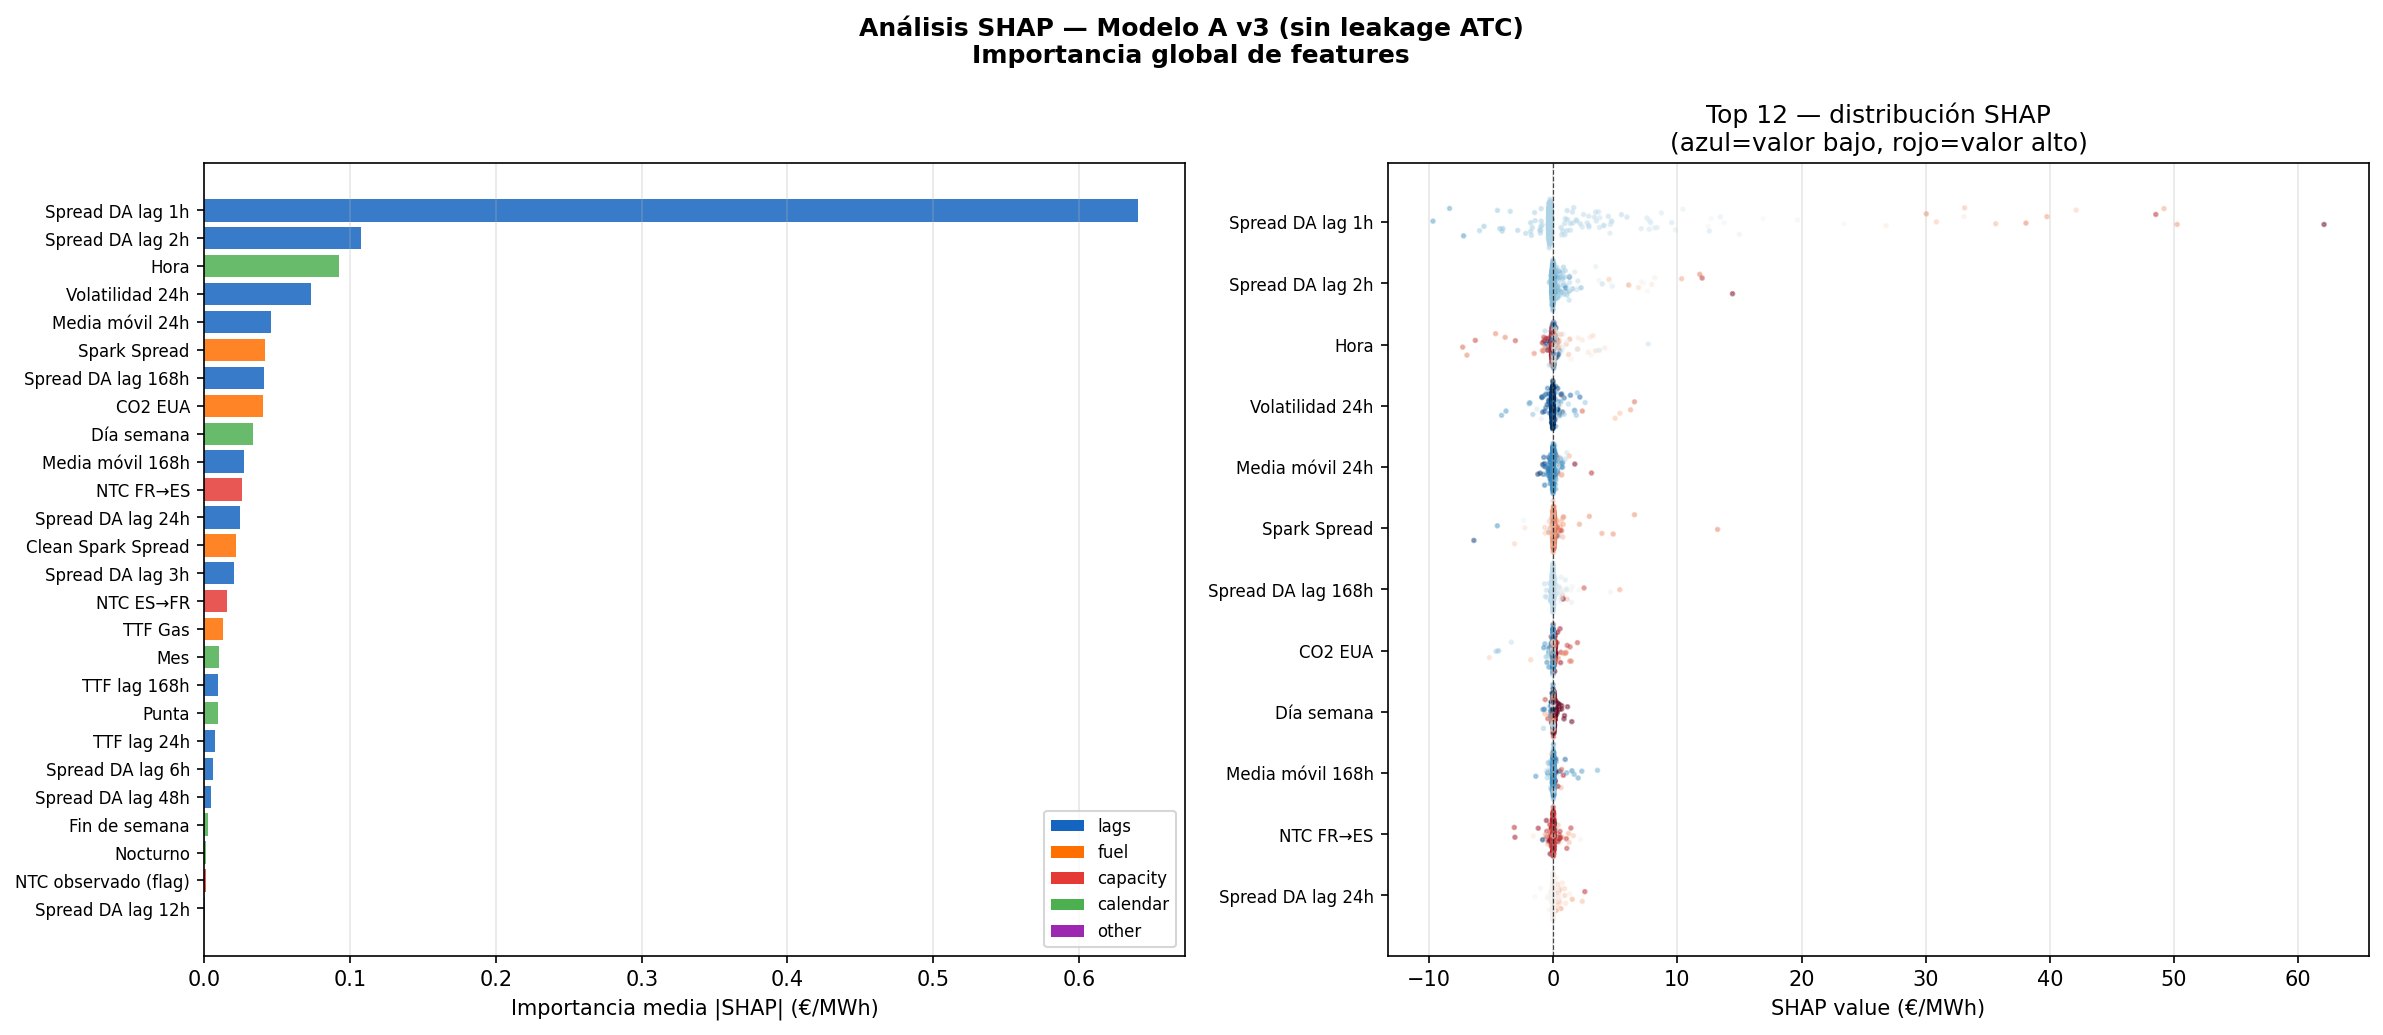
\includegraphics[width=0.95\linewidth]{08_shap_global_v3.png}
\caption{Global SHAP importance of Model A v3. Stratified sample by
regime, $n = 4\,998$.}
\label{fig:shap-global}
\end{figure}

The five dominant features are lags and recent volatility of the
spread; the spark spread appears as the eighth most important
feature. The interpretation is robust: the spread is a strongly
autocorrelated process at short horizons, and information from the
energy fundamentals reaches the prediction filtered through the lags.
This reading is consistent with the electricity-price-forecasting
literature \citep{Weron2014, Lago2021}.

\begin{figure}[H]
\centering
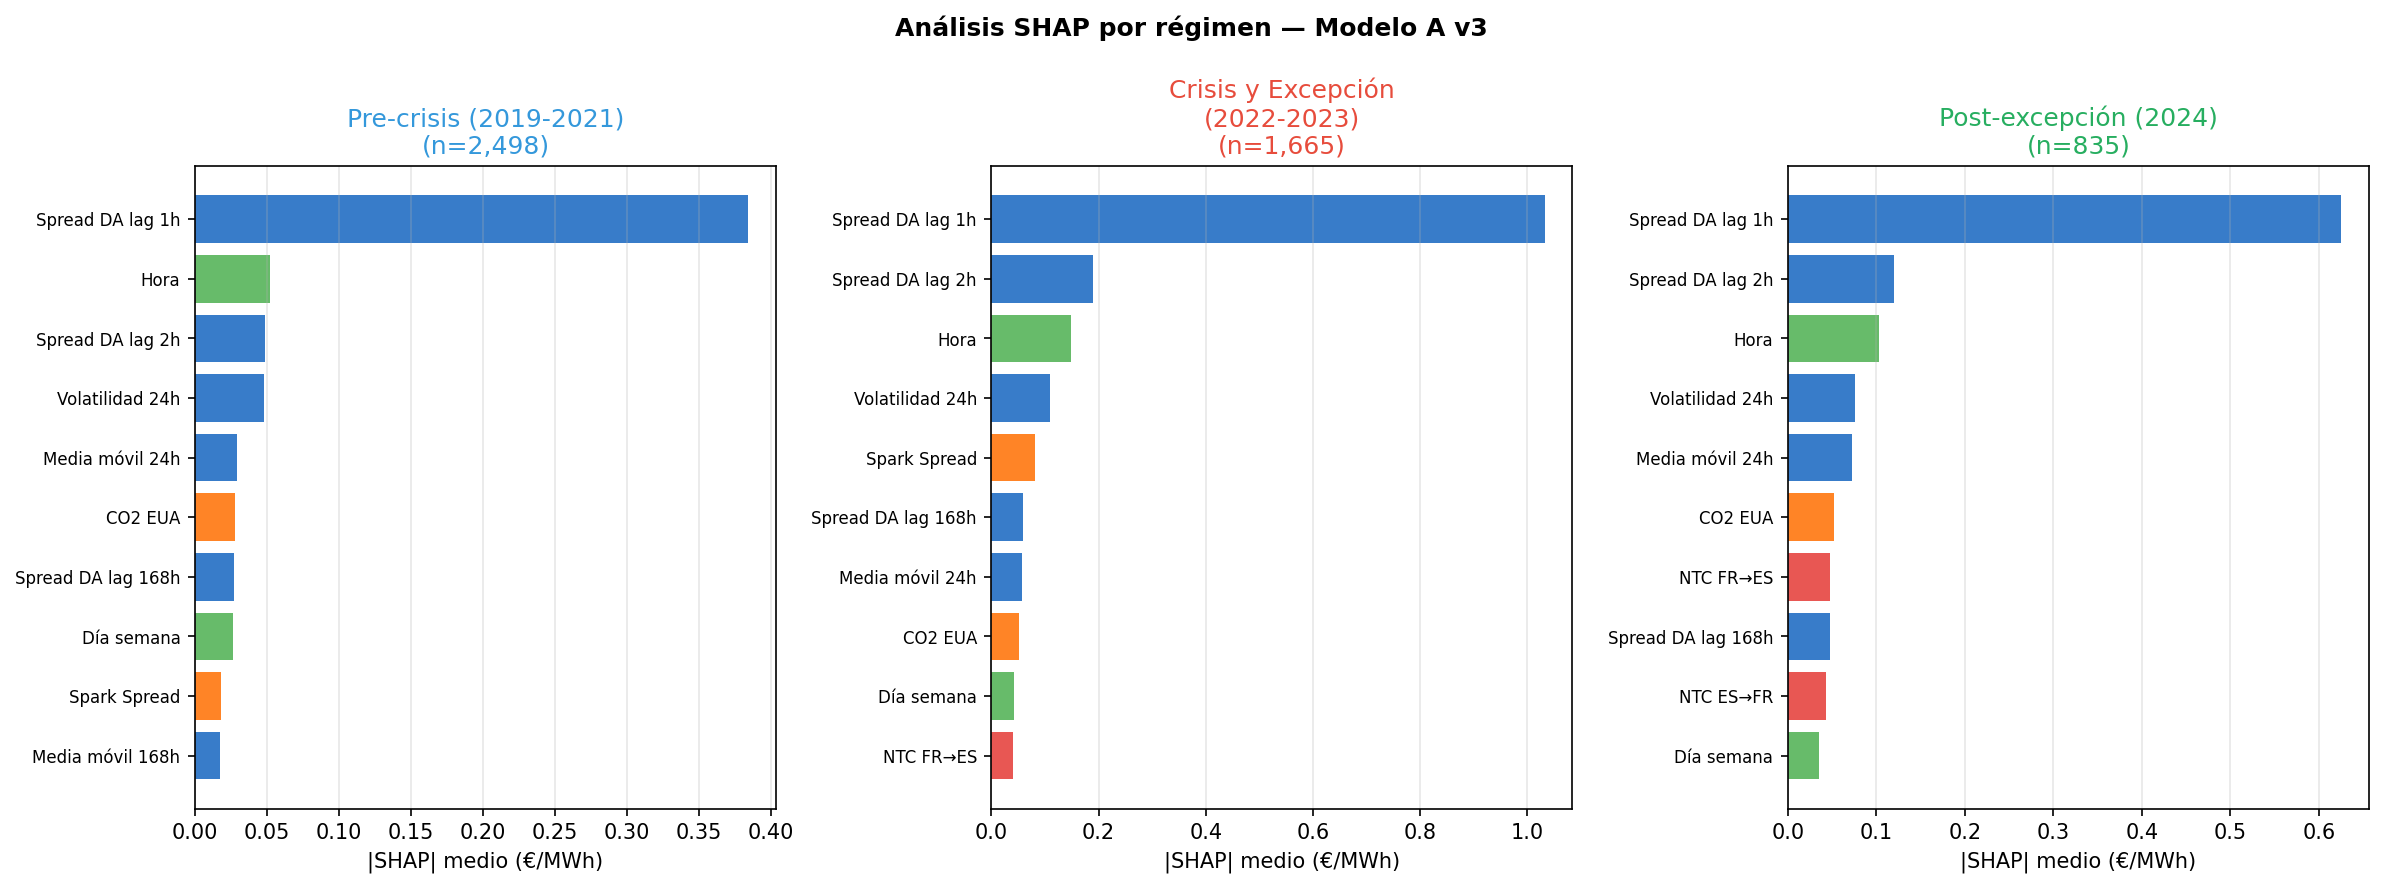
\includegraphics[width=0.95\linewidth]{09_shap_by_regime_v3.png}
\caption{SHAP importance by regime.}
\label{fig:shap-regime}
\end{figure}

\paragraph{Caveat on SHAP plots.} The SHAP feature-importance figures
above correspond to the Model A v3 trained before the rolling-feature
\texttt{shift(1)} correction described in the Note on revised metrics.
The qualitative ranking of features is expected to remain stable but
absolute $|\mathrm{SHAP}|$ values may shift slightly after
regeneration. SHAP regeneration is currently blocked by a documented
incompatibility between \texttt{shap} (versions 0.42--0.48) and
\texttt{xgboost} 3.2 in the JSON-model loading path; this is a
tooling issue, not a methodological one.

% =====================================================================
\section{Surveillance system and external validation}
% =====================================================================

\subsection{Anomaly detection --- operational definition}\label{sec:anomalies}

The residuals of Model A v3 feed the detection module. For each hour
$t$ the residual is normalised through a 168-hour \emph{rolling
z-score} with mandatory \texttt{shift(1)}, eliminating any possibility
of forward information leakage:
\[
z_t = \frac{r_t - \mu_{t-168 : t-1}}{\sigma_{t-168 : t-1}}.
\]
A numerical floor on the rolling standard deviation (10\% of the
global $\sigma$) and a symmetric clip on $z_t$ at $\pm 10$ prevent
artefactual amplification in low-volatility regimes; the share of
observations affected by either safeguard is reported in the audit
log.

\paragraph{Thresholds by regime.} The reference percentiles
($p_{90}$, $p_{95}$, $p_{99}$) are computed exclusively over the
\textbf{first 50\% temporal half of each regime} (training set).
This choice avoids look-ahead: the thresholds are fixed from the
early half of the regime and applied to the later period. The
estimated values are:

\begin{table}[H]
\centering
\small
\caption{$|z|$ thresholds calibrated on the first 50\% temporal half
of each regime.}
\label{tab:thresholds}
\begin{tabular}{lrrrr}
\toprule
\textbf{Regime} & \textbf{$p_{90}$} & \textbf{$p_{95}$} & \textbf{$p_{99}$} & \textbf{$n_\text{train}$} \\
\midrule
crisis\_y\_excepcion & 0{,}327 & 0{,}604 & 5{,}738 & 8\,705 \\
post\_excepcion      & 0{,}389 & 1{,}393 & 6{,}123 & 4\,349 \\
\bottomrule
\end{tabular}
\end{table}

(The \texttt{pre\_crisis} regime has no out-of-sample residuals by
construction of the expanding-window scheme and is reserved as
training data.)

\paragraph{Alert cascade.} The classification combines three
independent signals: the magnitude of the normalised residual ($|z|$),
multivariate statistical anomaly (Isolation Forest with régime-trained
percentile $p_{95}^{\mathrm{IF}} = 0{,}608$), and temporal persistence
(bilateral CUSUM with $\sigma$ estimated on the training set).

\begin{table}[H]
\centering
\small
\caption{Operational rules of the alert cascade.}
\label{tab:cascade}
\begin{tabular}{ll}
\toprule
\textbf{Level} & \textbf{Operational rule} \\
\midrule
Green   & $|z_t| < p_{90}$ \emph{and} IF\_score $< p_{95}$ \\
Amber   & $p_{90} \leq |z_t| < p_{95}$ \emph{or} IF\_score $\geq p_{95}$ \\
Orange  & $|z_t| \geq p_{95}$ \emph{and} (IF\_score $\geq p_{95}$ \emph{or} CUSUM active) \\
Red     & $|z_t| \geq p_{99}$ \emph{and} IF\_score $\geq p_{95}$ \emph{and} CUSUM persistent $\geq 3$h \\
\bottomrule
\end{tabular}
\end{table}

The Red level requires the simultaneous confirmation of three
independent criteria. Each classification is recorded with
\texttt{(timestamp, $z_t$, if\_score, cusum\_state, level)} for full
auditability.

\paragraph{Table~\ref{tab:t4}: distribution of alerts.} Alerts are
computed over the hours with available out-of-sample prediction
(approximately $26\,277$~hours, 2022--2024). The 2019--2021 period
is exclusively training and by construction does not produce alerts;
any reference to ``2019--2024 alerts'' should be read as ``alerts in
the sub-period with out-of-sample prediction''.

\begin{table}[H]
\centering
\small
\caption{Table 4 --- Distribution of alerts (Model A v3, cascade v3).}
\label{tab:t4}
\begin{tabular}{lrr}
\toprule
\textbf{Level} & \textbf{Hours} & \textbf{\% of classified} \\
\midrule
Green   & 23\,358 & 88{,}89 \\
Amber   &  2\,168 &  8{,}25 \\
Orange  &     690 &  2{,}63 \\
Red     &      61 &  0{,}23 \\
\midrule
\textbf{Total classified} & \textbf{26\,277} & \textbf{100{,}00} \\
\bottomrule
\end{tabular}
\end{table}

\begin{figure}[H]
\centering
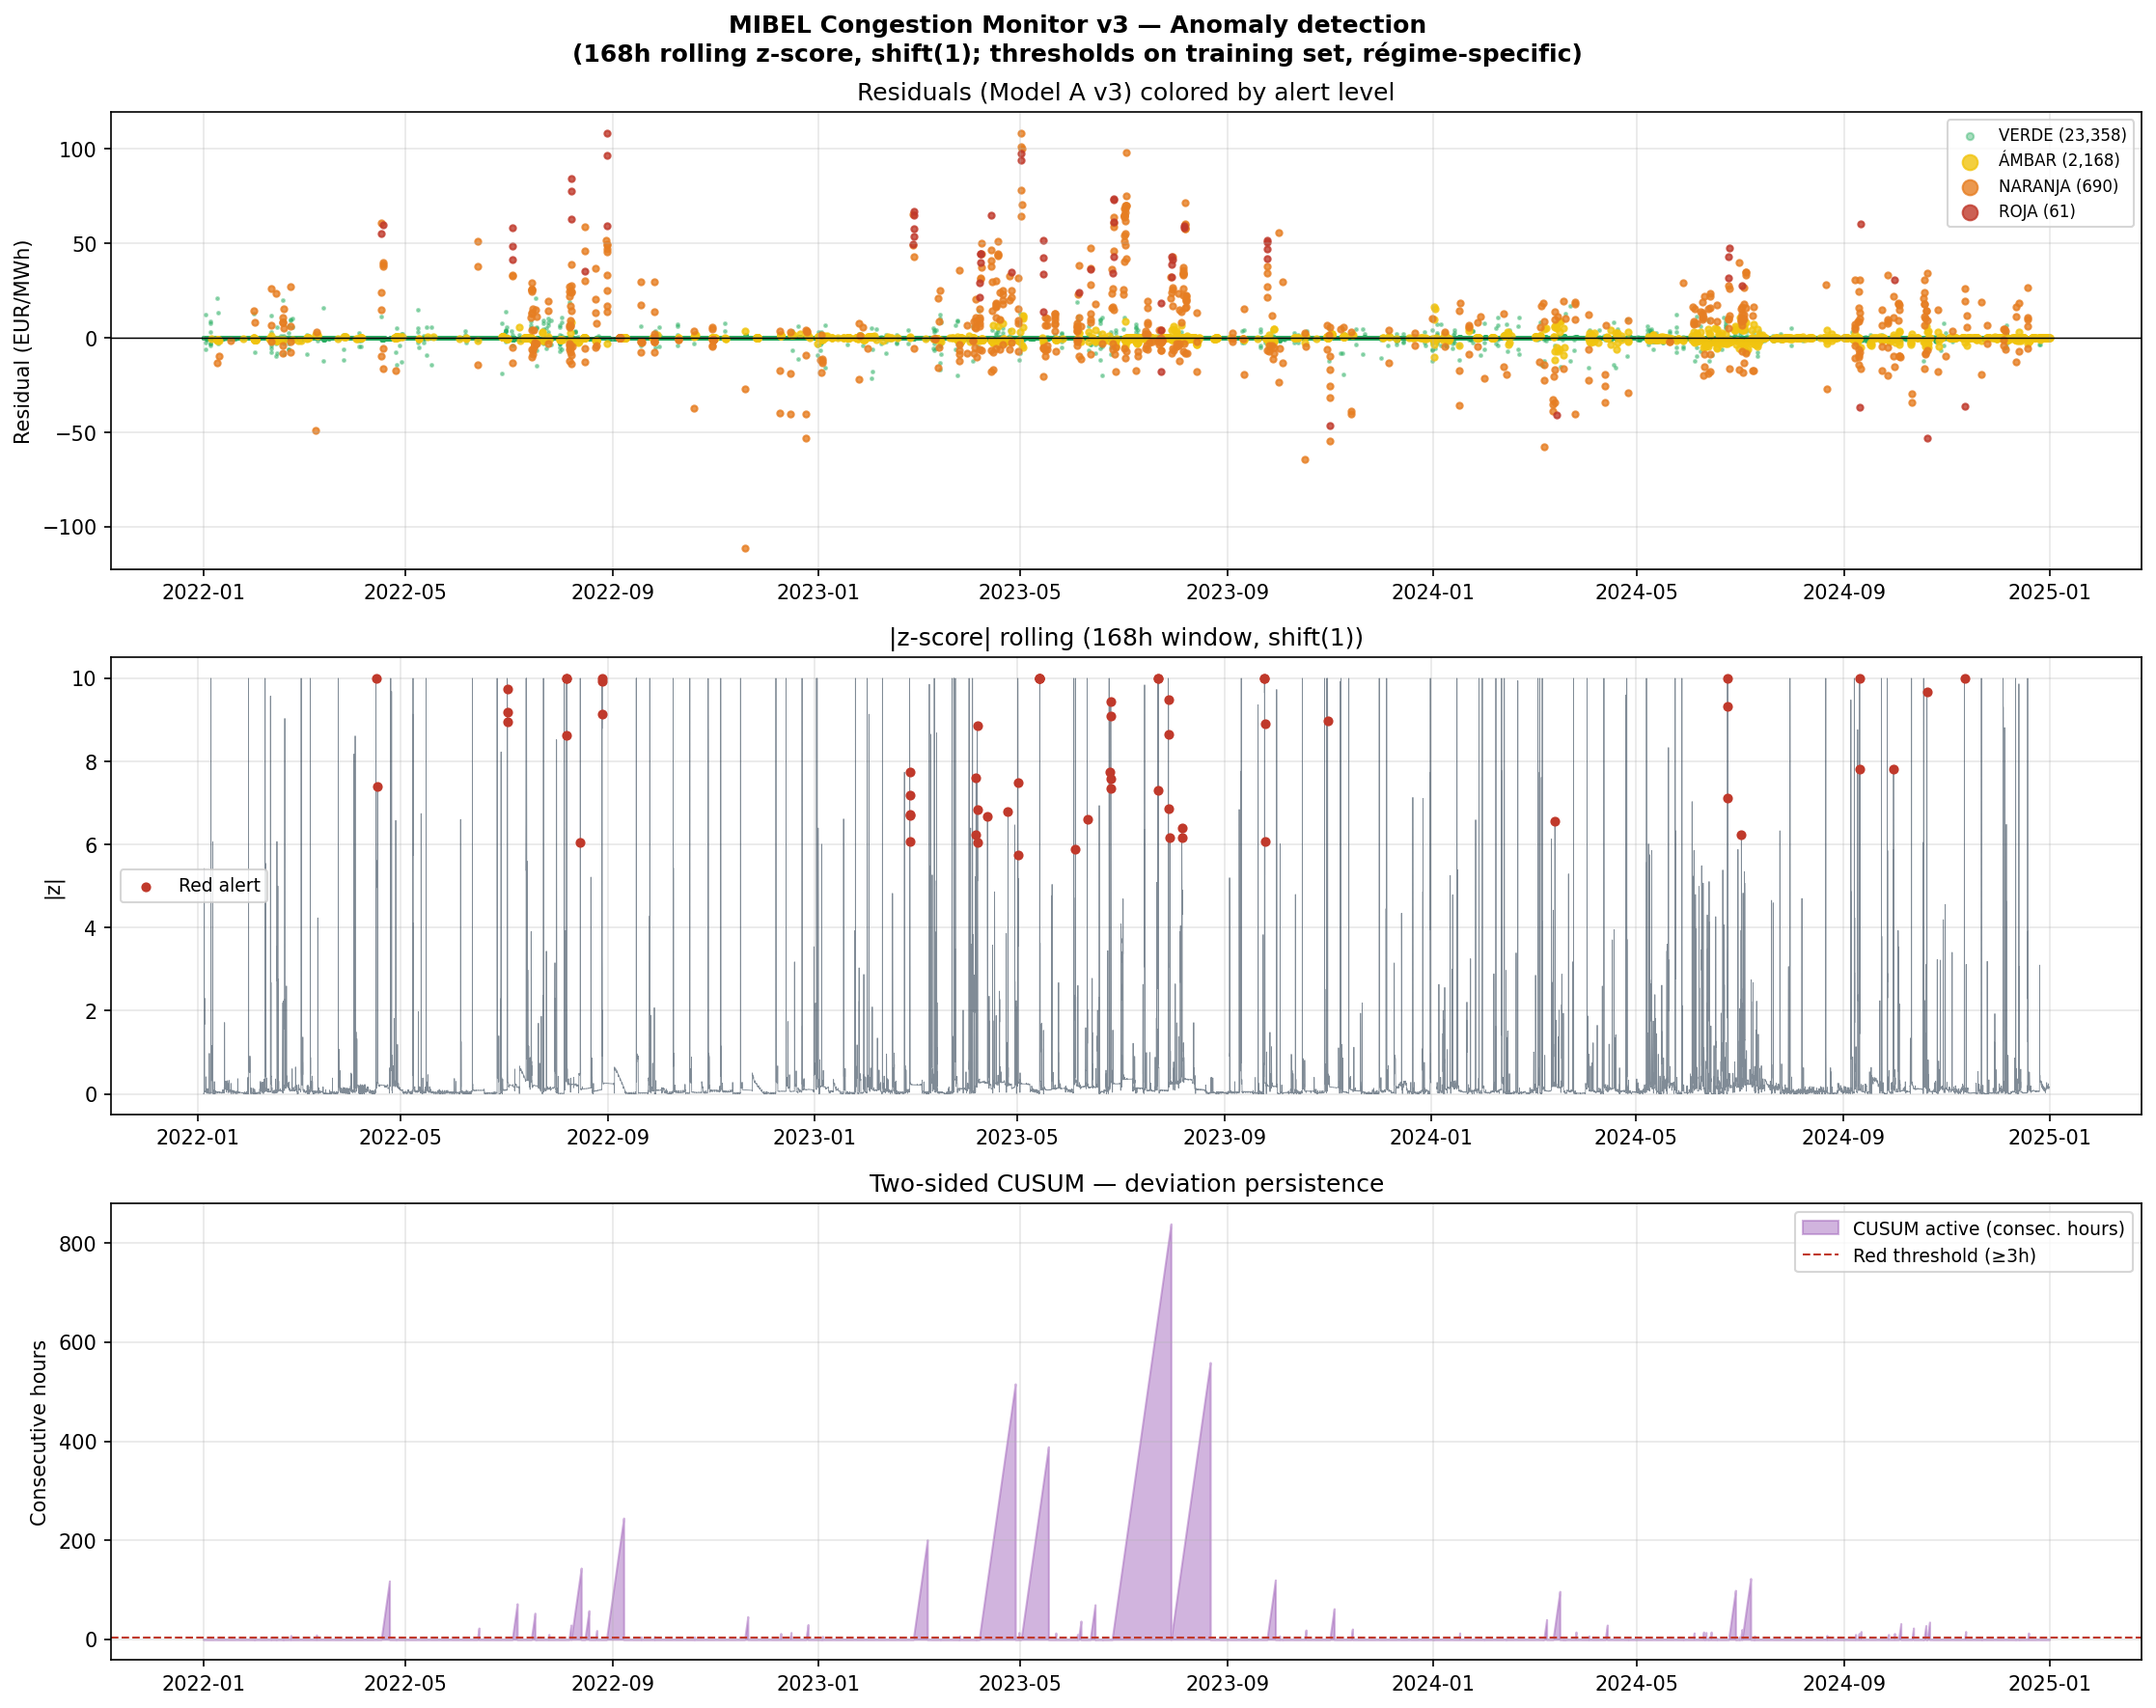
\includegraphics[width=0.95\linewidth]{06_anomaly_detection_v3.png}
\caption{Anomaly detection on the residuals of Model A v3.}
\label{fig:anomaly-detection}
\end{figure}

\subsection{Three illustrative episodes}\label{sec:illustrative}

For qualitative purposes, three Red-alert episodes are contrasted
against documented events:

\begin{enumerate}
\item \textbf{28 August 2022} (residual $\approx 59{,}4$~€/MWh):
historical minimum of French nuclear generation since 1992
\citep{RTE2023}; Spain exports at the maximum interconnection
capacity, amplified by the Iberian Exception.

\item \textbf{1 May 2023} (residual $\approx 97{,}4$~€/MWh):
national holiday with minimum demand in Spain, high renewable
generation, active gas-cap regime \citep{OMIE2023}.

\item \textbf{July 2023} (seven Red Alerts recorded):
European heat wave, cooling demand in France, contained prices in
Spain \citep{CNMC2024}.
\end{enumerate}

These three episodes illustrate the system's response to high-profile
documented events. The systematic validation against the complete
event panel is reported in Section~\ref{sec:event-validation}.

\subsection{Systematic validation against the event panel}\label{sec:event-validation}

To avoid the \emph{post-hoc} bias inherent in the manual selection of
episodes, we construct a pre-specified panel of 40 verified events
from the Iberian--European electricity market between 2019 and 2024,
coded by type (\texttt{MERCADO}, \texttt{INFRAESTRUCTURA},
\texttt{CLIMATICO}, \texttt{REGULATORIO}, \texttt{LABORAL},
\texttt{GEOPOLITICO}), magnitude (LOW/MEDIUM/HIGH/VERY HIGH),
direction of impact and primary sources.

\paragraph{Panel design.} The panel is \emph{structural} by design:
event metadata are encoded as categorical codes
(\texttt{event\_type}, \texttt{magnitude\_indicator},
\texttt{direction\_impact}) rather than free-text descriptions. The
\texttt{event\_name} and \texttt{description\_es} fields are
intentionally left blank or coded with the event identifier to
ensure reproducible categorisation and to prevent ambiguity in
event classification.

\paragraph{Operational definition.} An event is considered
\textbf{detected} if at least one hour within
$[\text{date\_start}, \text{date\_end}]$ produces an Orange or Red
alert from the system. As a baseline benchmark, we compare against a
naive rule: alert if $|\mathrm{spread}_\text{DA}| > p_{99}$ of the
corresponding regime (computed over the full regime).

\paragraph{Coverage.} Of the 40 panel events, $24$ fall fully or
partially within the alert window (2022--2024); the $16$ events of
2019--2021 are out-of-window by construction of the expanding-window
scheme.

\begin{table}[H]
\centering
\small
\caption{Table 5 --- Recall by magnitude (in-window events 2022--2024).}
\label{tab:t5}
\begin{tabular}{lrrrrr}
\toprule
\textbf{Magnitude} & \textbf{Total} & \textbf{In-window} & \textbf{Detected} & \textbf{System recall} & \textbf{Naive recall} \\
\midrule
VERY HIGH & 14 & 8 & 7 & \textbf{0{,}875} & 0{,}750 \\
HIGH      & 16 & 9 & 6 & 0{,}667 & 0{,}667 \\
MEDIUM    &  9 & 6 & 6 & \textbf{1{,}000} & 0{,}833 \\
LOW       &  1 & 1 & 1 & 1{,}000 & 1{,}000 \\
\midrule
\textbf{Total} & 40 & 24 & 20 & \textbf{0{,}833} & 0{,}750 \\
\bottomrule
\end{tabular}
\end{table}

\begin{table}[H]
\centering
\small
\caption{Table 6 --- Recall by event type (in-window).}
\label{tab:t6}
\begin{tabular}{lrrrrr}
\toprule
\textbf{Type} & \textbf{Total} & \textbf{In-window} & \textbf{Detected} & \textbf{System recall} & \textbf{Naive recall} \\
\midrule
MERCADO         & 22 & 13 & 11 & \textbf{0{,}846} & 0{,}692 \\
INFRAESTRUCTURA &  6 &  4 &  4 & 1{,}000 & 1{,}000 \\
CLIMATICO       &  5 &  2 &  2 & 1{,}000 & 1{,}000 \\
REGULATORIO     &  4 &  2 &  1 & 0{,}500 & 0{,}500 \\
LABORAL         &  2 &  2 &  2 & 1{,}000 & 1{,}000 \\
GEOPOLITICO     &  1 &  1 &  0 & 0{,}000 & 0{,}000 \\
\bottomrule
\end{tabular}
\end{table}

\begin{table}[H]
\centering
\small
\caption{Table 7 --- System (cascade v3) vs naive benchmark
($|\mathrm{spread}| > p_{99}$ regime). Detection overlap over 24
in-window events.}
\label{tab:t7}
\begin{tabular}{lrr}
\toprule
\textbf{Category} & \textbf{System v3} & \textbf{Naive $p_{99}$} \\
\midrule
Detections (in-window)         & 20 & 18 \\
Recall global (in-window)        & \textbf{0{,}833} & 0{,}750 \\
\midrule
\textbf{Overlap}                 & \multicolumn{2}{c}{$n$} \\
\midrule
Both detect                      & \multicolumn{2}{c}{18} \\
Only system                      & \multicolumn{2}{c}{2} \\
Only naive                       & \multicolumn{2}{c}{0} \\
Neither                          & \multicolumn{2}{c}{4} \\
\bottomrule
\end{tabular}
\end{table}

\paragraph{Honest reading.} The system outperforms the naive
benchmark by $+8{,}3$ percentage points of recall ($0{,}833$ vs
$0{,}750$) and \emph{never misses an event detected by the naive
benchmark}: it adds two detections that the naive benchmark misses,
without losing any. The advantage is modest but systematic; with
$n = 24$ the paired McNemar test does not reach 5\% significance
(the asymmetry is 2 vs 0 in the discordant cells, $p = 0{,}500$ in
the two-sided exact test). The Wilson CI95\% for the system recall
is $[0{,}641;\, 0{,}933]$; for the naive benchmark it is
$[0{,}551;\, 0{,}880]$. The intervals overlap substantially,
consistent with the non-significance of the McNemar test. The
cautious conclusion is: the system adds information beyond the raw
spread, but the statistical power of the current panel does not
permit a formal claim of dominance.

\paragraph{Additional operational metrics.} Beyond detection
parity, the system is characterised by precision and lead-time
metrics that quantify its operational utility:
\begin{itemize}
\item \textit{Precision@72h} (alerts within $\pm 72$~hours of a
documented event centre): $0{,}148$.
\item \textit{Precision@7d}: $0{,}205$.
\item \textit{Precision@30d}: $0{,}783$.
\item \textit{False-positive rate per month outside $\pm 72$~h}:
$17{,}9$ alerts/month.
\item \textit{Recall within 24h} of event onset: $0{,}167$.
\item \textit{Recall within 48h}: $0{,}208$.
\item \textit{Recall within 168h} (one week): $0{,}417$.
\item \textit{Median lag} between event onset and first alert:
$180$~h ($\approx 7{,}5$ days).
\item \textit{75th percentile lag}: $313$~h ($\approx 13$ days).
\end{itemize}

The median lag of 180~hours indicates that the system functions as a
retrospective filter rather than as an operational early-alert
mechanism. Only 21\% of detected events are captured in the first
48 hours of the documented onset. This is an operationally relevant
limitation for REMIT~II surveillance that requires early action.

\paragraph{Failure analysis.} The four VERY HIGH / HIGH in-window
events that the system misses are:

\begin{itemize}
\item \textbf{EVT019 (VERY HIGH, GEOPOLITICAL)} --- Russian invasion
of Ukraine: a global, persistent energy shock that enters the
\texttt{crisis\_y\_excepcion} regime from its start; the model
absorbs the new level through lags and produces no alert because the
residual has already stabilised by the time the regime begins.
\item \textbf{EVT033 (HIGH, REGULATORY)} --- End of the Iberian
Exception: a convergence expected by the model's construction. The
system is designed to detect \emph{divergence} from the expected
behaviour; the post-Exception convergence is consistent with the
fundamentals and should not trigger an alert. This is a
\emph{correct miss}: the event is real but is not an anomaly in the
residual sense.
\item \textbf{EVT035 / EVT036 (HIGH, MARKET)} --- Sporadic negative
prices in Spain (1 April 2024 and 20 April 2024): affect the
absolute price but not necessarily the bilateral spread if France
moves in the same direction.
\end{itemize}

\paragraph{Limitation of the panel.} With $n = 40$ events over six
years (24 in-window), statistical power is limited for rare
magnitudes (LOW with $n = 1$ does not permit inference). A natural
extension is to expand the panel with REE/ESIOS incident codes and
CNMC technical notes encoded at hourly granularity.

\begin{figure}[H]
\centering
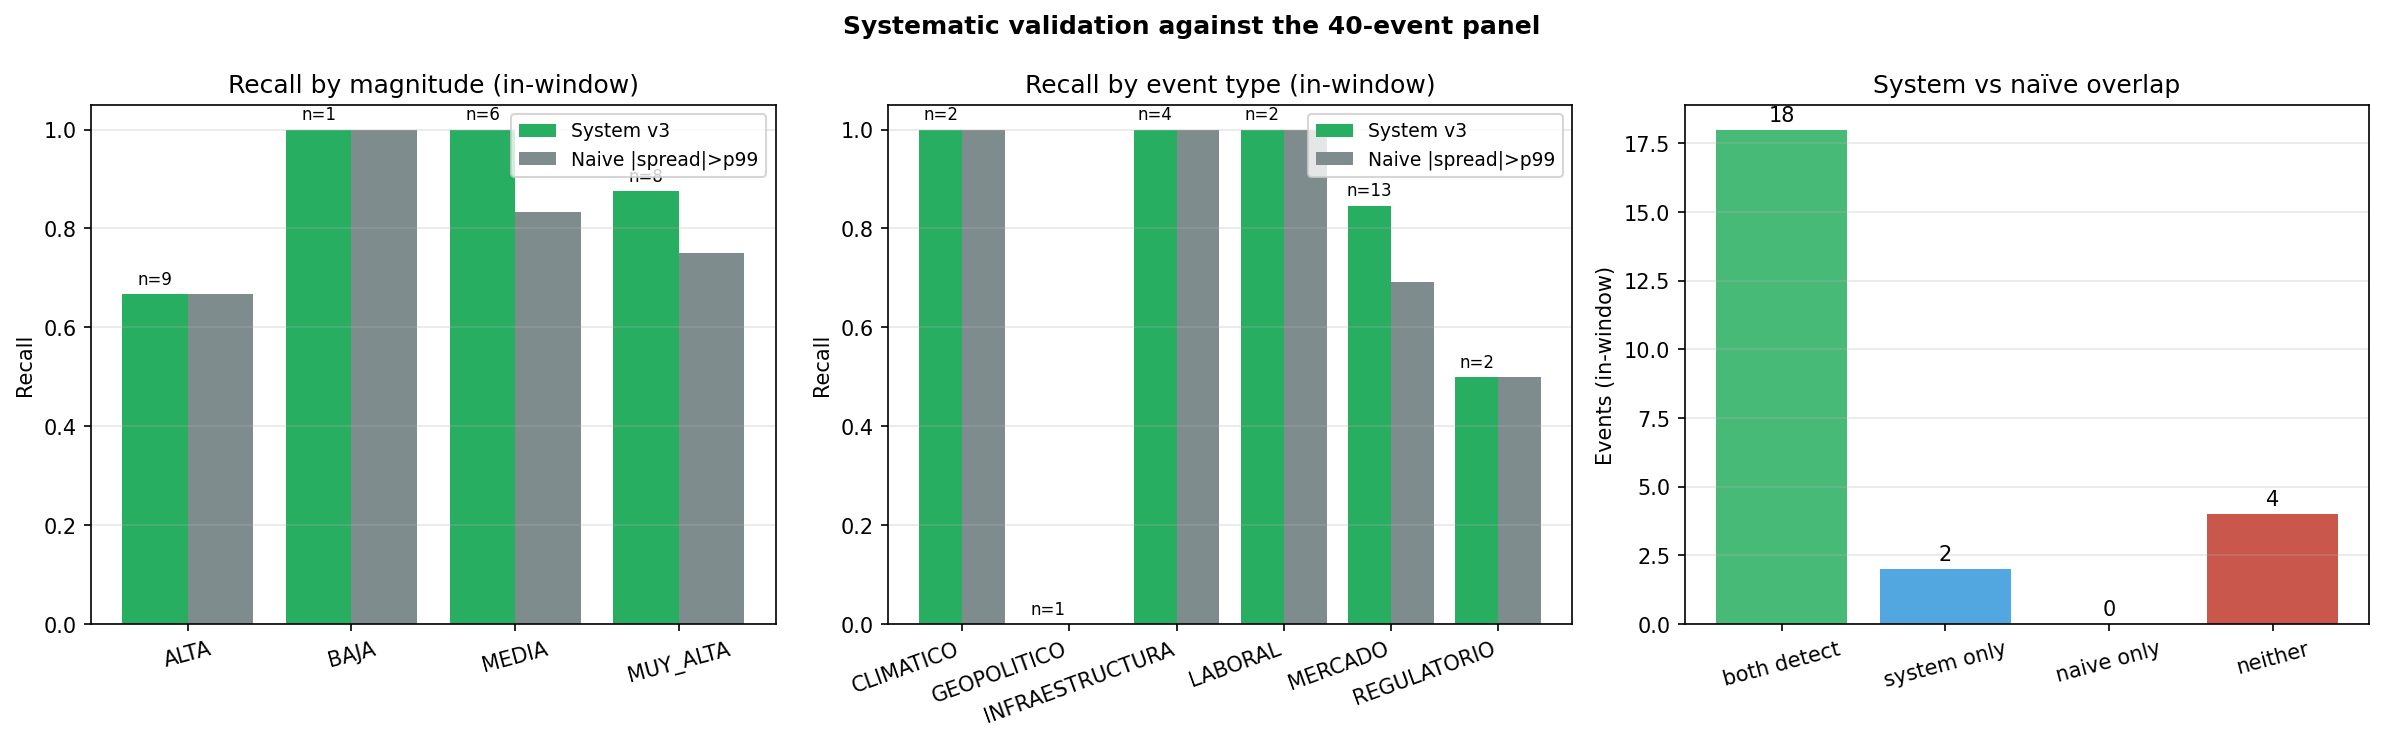
\includegraphics[width=0.95\linewidth]{event_validation.png}
\caption{Systematic validation against the 40-event panel.}
\label{fig:event-validation}
\end{figure}

% =====================================================================
\section{Operational calibration: precision-coverage trade-off}\label{sec:opcal}
% =====================================================================

Beyond a single fixed operating point, the cascade admits
recalibration to the analytical capacity of the regulator. We
construct a grid of 100 threshold combinations (5 z-score
régime-specific percentiles $\times$ 5 IsolationForest percentiles
$\times$ 4 CUSUM persistence thresholds, all computed out-of-sample
on the training fraction) and evaluate each configuration on four
metrics: monthly alert volume, precision@72h, recall@event, and the
false-positive rate outside the 72-hour window around documented
event centres. The resulting Pareto frontier
(Figure~\ref{fig:pareto}) exhibits a clear elbow at approximately
4--5 alerts per month: configurations below this volume lose
coverage substantially, while configurations above dilute precision
without recovering recall.

\begin{table}[H]
\centering
\small
\caption{Operational calibration: four canonical capacity points
from the OOS grid plus the current in-sample operating point.}
\label{tab:opcal}
\begin{tabular}{lcccccc}
\toprule
\textbf{Capacity} & \textbf{Alerts/mo.} & \textbf{$z$-thr.} & \textbf{IF-thr.} & \textbf{CUSUM} & \textbf{Recall@event} & \textbf{Precision@72h} \\
\midrule
Very low                  & 2{,}1 & $p_{99{.}5}$ & $p_{90}$ & $\geq 1$h & 0{,}833 & 0{,}182 \\
\textbf{Low (elbow)}      & \textbf{4{,}3} & $p_{99}$    & $p_{90}$ & $\geq 1$h & \textbf{0{,}833} & \textbf{0{,}212} \\
Medium                    & 12{,}2 & $p_{97}$   & $p_{80}$ & $\geq 1$h & 0{,}833 & 0{,}169 \\
High                      & 19{,}7 & $p_{93}$   & $p_{80}$ & $\geq 1$h & 0{,}833 & 0{,}168 \\
\midrule
Current (in-sample IF)    & 20{,}9 & $p_{99}$ OOS & $p_{95}$ IS global & $\geq 3$h & 0{,}833 & 0{,}148 \\
\bottomrule
\end{tabular}
\end{table}

The system's default operating point (20{,}9 alerts/month,
precision@72h $= 0{,}148$) lies above the elbow and is dominated by
the ``Low capacity'' calibration (4{,}3 alerts/month,
precision@72h $= 0{,}212$): both produce identical coverage
(recall@event $= 0{,}833$) over the 24 in-window events, but the
elbow configuration improves precision by 43\% and reduces alert
volume by a factor of five. A CNMC or ACER analyst with approximately
2 hours per week of dedicated review capacity could process the
elbow configuration without coverage loss.

\paragraph{CUSUM persistence and IF in-sample threshold.}
Two calibration choices contribute to the default's position above
the elbow: (i) a CUSUM persistence threshold of 3 hours, and (ii) the
use of an in-sample, regime-pooled IF percentile rather than the
régime-specific out-of-sample percentile used in the grid. Across all
canonical operating points selected by the Pareto analysis, the
dominant CUSUM persistence threshold is 1 hour: configurations
requiring longer persistence discard alerts that would maintain
recall without improving precision. We retain CUSUM as a noise
filter to prevent isolated z-score spikes from triggering alerts,
but recommend setting minimum persistence to 1 hour rather than 3.

\paragraph{Regulatory positioning.} This calibration is reported as
guidance for capacity-adjusted deployment rather than as a
substitute for the default cascade. The system functions as a
\emph{quantitative screening layer}, not as a regulatory imputation
mechanism: its output identifies hours warranting investigation by
analysts with access to additional information (aggregate supply
curves, operator positions, operational context) outside the scope
of this work. A Red alert from the system does not constitute
evidence of market manipulation; it identifies an episode whose
price dynamics are not explained by the contemporaneous
fundamentals and whose duration, direction, and persistence merit
human review.

\begin{figure}[H]
\centering
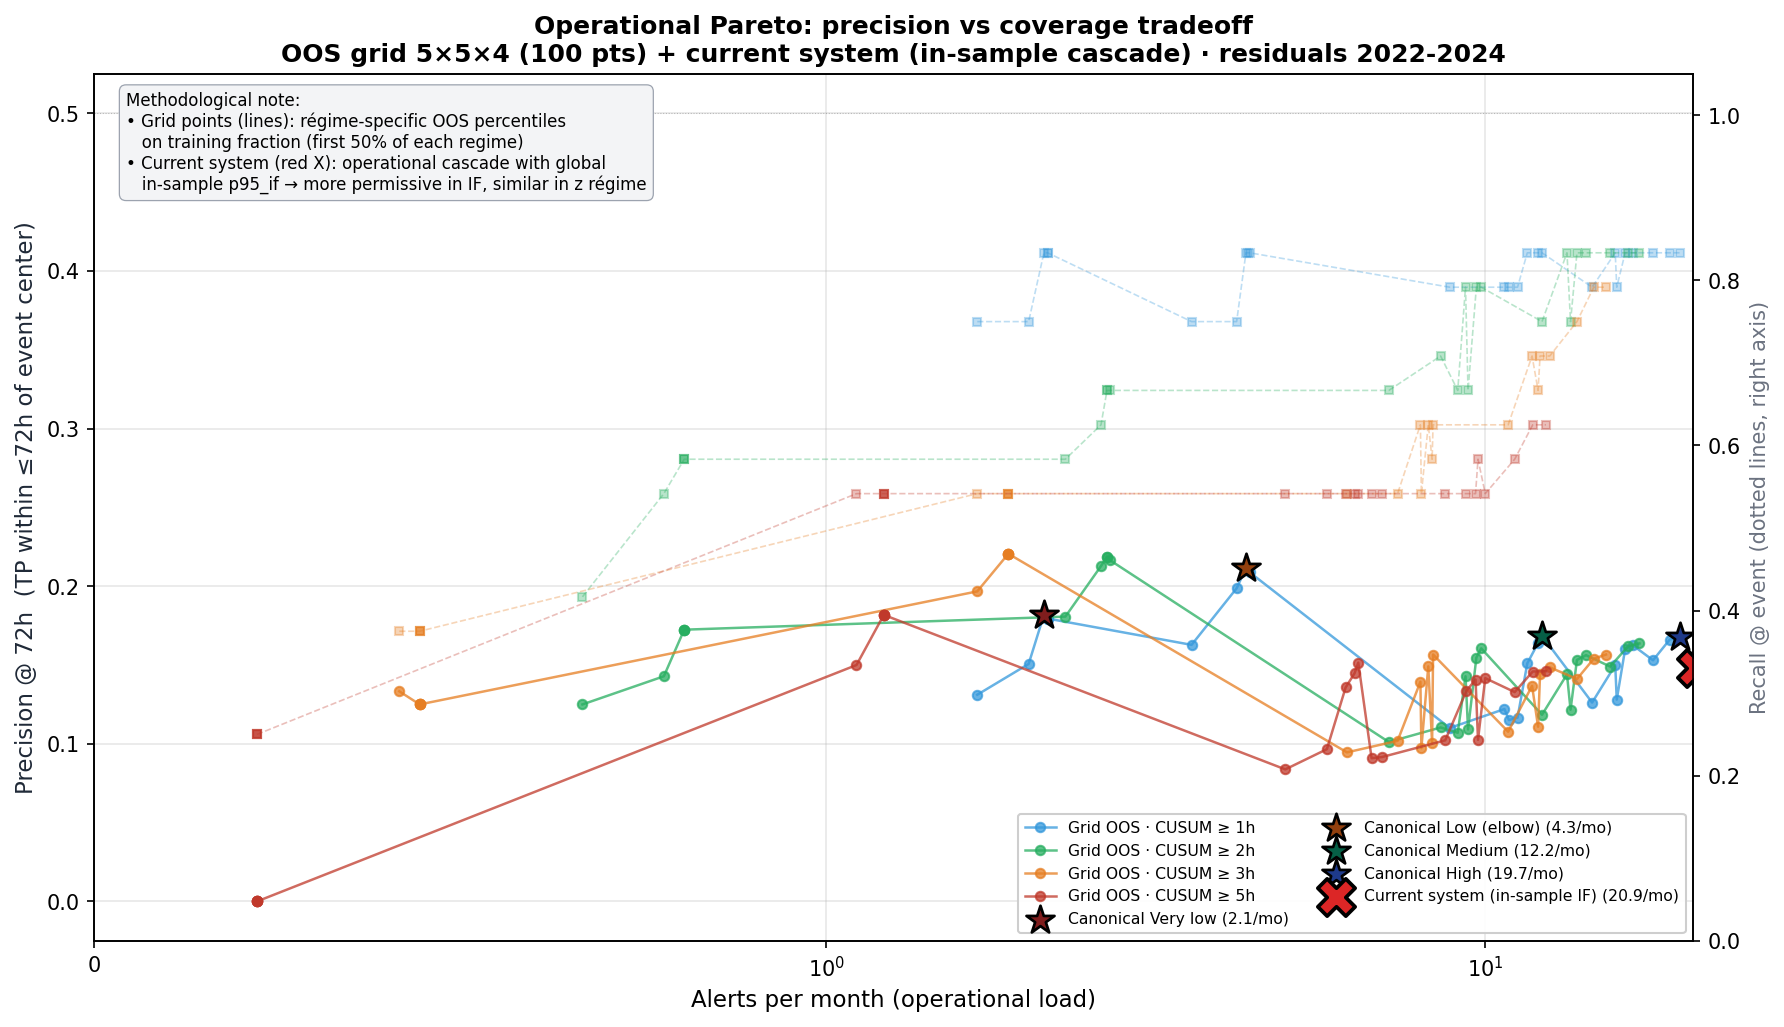
\includegraphics[width=0.95\linewidth]{10_operational_calibration_pareto.png}
\caption{Pareto frontier of precision @ 72h vs alert volume across
100 threshold combinations. Lines correspond to different CUSUM
persistence thresholds (1, 2, 3, 5 hours). The system's current
operating point (red X marker) lies above the elbow at
$\sim 4$--$5$ alerts/month. Canonical operating points for four
capacity bands are labeled (Very low, Low/elbow, Medium, High).}
\label{fig:pareto}
\end{figure}

% =====================================================================
\section{Limitations}\label{sec:limitations}
% =====================================================================

\paragraph{Coverage of the alert system.} The
Green/Amber/Orange/Red cascade is computed over the out-of-sample
residuals of the expanding-window scheme, which limits the
operational window to the 2022--2024 period
($\sim 26\,000$~hours). The 2019--2021 period is exclusively
training and by construction does not produce alerts; a
qualitatively analogous validation over that sub-period would
require a block-wise temporal cross-validation strategy.

\paragraph{Statistical power of the event panel.} With $n = 40$
verified events over six years (24 in-window), the asymmetry of the
McNemar test between the system and the naive benchmark does not
reach 5\% significance. Expansion to denser panels (REE/ESIOS
incident codes and CNMC technical notes at hourly granularity) is
the natural path to give formal power to the finding.

\paragraph{Benchmark coverage.} The reported benchmarks cover simple
autoregressive models (AR(1), AR(24)) and regularised linear models
(LASSO). Models with explicit seasonality (SARIMA with daily and
weekly components) are not included in this version; similar
behaviour is expected given that the seasonal components are captured
implicitly via the calendar features in the main model.

\paragraph{Data sources for fundamentals.} The use of
\texttt{yfinance} for TTF and EUA is practical but does not
constitute a primary regulatory source. A serious operational
deployment would require a subscription to Euronext/EEX (TTF) or ICE
Endex (EUA).

\paragraph{SHAP interpretability under correlation.} Tree-SHAP can
be biased in the presence of correlated features \citep{Lago2021}.
In this system, spread lags, volatility and energy fundamentals are
partially correlated; SHAP values should be read as descriptive
attribution, not causal identification. Additionally, as noted in
the SHAP caveat above, the figures are derived from a model trained
before the rolling-feature \texttt{shift(1)} correction; the
qualitative ranking is expected to remain stable but absolute
$|\mathrm{SHAP}|$ values may shift slightly after regeneration.

\paragraph{Regime dating.} The \texttt{crisis\_y\_excepcion} regime
aggregates January--14 June 2022 (crisis without cap) and 15 June
2022--31 December 2023 (Iberian Exception) for sample-size reasons.
Formal regime-switching models (Markov-switching) on the exact date
of Royal Decree-Law~10/2022 are a natural extension but require
additional sample size in each sub-regime.

\paragraph{Lead time of detection.} The median lag between the
documented event onset and the first system alert is approximately
$7{,}5$ days ($180$~h), with the 75th percentile at $13$ days
($313$~h). Only 21\% of in-window events are detected within 48
hours and 17\% within 24 hours. This positions the system as a
retrospective surveillance and forensic screening tool rather than
a real-time alert mechanism. The lag is consistent with the
day-ahead nature of the underlying market (daily auction, not
continuous trading) and with the structural duration of detected
episodes (heat waves, regulatory shocks, generation restrictions
develop over days or weeks). Real-time surveillance would require
intraday continuous-market data (XBID) and a substantially different
methodology.

\paragraph{Overcalibration of the default cascade.} The default
cascade configuration analysed in Section~\ref{sec:anomalies}
operates above the Pareto elbow identified in
Section~\ref{sec:opcal} (operational calibration). This reflects
two calibration inheritances from earlier versions of the pipeline:
the in-sample IF percentile and the 3-hour CUSUM persistence
threshold. The default is preserved in the reported artefacts for
consistency with the experimental design; the elbow configuration
is reported as the recommended operational deployment.

% =====================================================================
\section{Conclusions and next steps}
% =====================================================================

The project explores the feasibility of a residual indicator derived
from economic fundamentals as input to a broader market-surveillance
system. The main findings are:

\begin{enumerate}
\item \textbf{The residual as signal.} On the 2024 test set the
fundamentals model achieves $R^2 = 0{,}539$ (notably modest with
respect to the literature on zonal pricing but consistent with the
intra-day noise of bilateral spreads) and the residuals carry
incremental information over the raw spread, materialised in a
conservative cascade of $61$~Red Alerts over 2022--2024 (default
cascade).

\item \textbf{Main model vs competitive benchmarks.} The XGBoost
achieves lower RMSE than the AR(1), AR(24) and LASSO benchmarks on
the 2024 test ($3{,}218$ vs $3{,}424/3{,}427/3{,}376$~€/MWh), but
the Diebold--Mariano test does not reach 5\% significance with
$n = 8\,783$ ($p \in [0{,}06;\,0{,}12]$). Statistical significance
is maintained only against the naive benchmarks of persistence and
zero level ($p < 10^{-3}$). The model's operational advantage
concentrates in the tail of the distribution rather than in the
average fit, aligned with its surveillance use.

\item \textbf{Modest but positive external validation.} Against a
pre-specified panel of 40 verified events, the system detects 83\%
of in-window events, against 75\% of a naive benchmark on
$|\mathrm{spread}|$ at the régime-specific $p_{99}$ threshold. The
advantage is $+8{,}3$~p.p. but $n = 24$ does not deliver formal
significance (McNemar $p = 0{,}500$; Wilson CI95\% for the system
recall: $[0{,}641;\,0{,}933]$). The system improves detection without
losing any event the naive benchmark detects; the power of the
current panel is limited.

\item \textbf{Régime-specific models.} The régime-specific
specification outperforms the unified pooled model by an ample
margin in \texttt{crisis\_y\_excepcion} ($-18{,}1\%$ RMSE), while
in \texttt{pre\_crisis} and \texttt{post\_excepcion} both
specifications are in technical tie ($<2\%$ RMSE in either
direction). The evidence rules out the strong hypothesis of
transfer learning dominating across regimes and reinforces the
relevance of régime-specific models for non-stationary regulatory
periods.

\item \textbf{Operational calibration is a substantive degree of
freedom.} The default cascade operates above the Pareto elbow of
the precision-coverage trade-off. The elbow configuration (4{,}3
alerts/month) achieves the same coverage at five times lower
operational load and 43\% higher precision@72h; this is reported as
guidance for capacity-adjusted deployment, not as a substitute for
the default cascade.
\end{enumerate}

\paragraph{Next steps.} (i)~Integration of hourly demand
(REE/ESIOS) and aggregate supply data (PMD/ESIOS) to enrich the
feature set. (ii)~Adaptation to the quarter-hourly resolution of
MIBEL deployed in 2025. (iii)~Expansion of the event panel to
hourly granularity through encoding of CNMC technical notes and
OMIE/REE bulletins. (iv)~Replacement of TTF/EUA from
\texttt{yfinance} by licensed Euronext/EEX sources.
(v)~Formal regime-switching models (Markov-switching) instead of
calendar-based regulatory splits. (vi)~Adoption of the Pareto-elbow
calibration ($z_{p_{99}}$ régime-specific, $\mathrm{IF}_{p_{90}}$
out-of-sample, $\mathrm{CUSUM} \geq 1$h) as the default operational
configuration, replacing the current in-sample calibration. This
recalibration preserves recall@event and improves precision@72h
from $0{,}148$ to $0{,}212$ with a five-fold reduction in alert
volume.

% =====================================================================
\bibliographystyle{apalike}
\bibliography{refs}

\end{document}
